\begin{enumerate}[label=\thesection.\arabic*,ref=\thesection.\theenumi]
\numberwithin{equation}{enumi}
\numberwithin{figure}{enumi}
\item
\label{12/12/1/1}
%\iffalse
\documentclass[journal,10pt,twocolumn]{article}
\usepackage{graphicx}
\usepackage[margin=0.5in]{geometry}
\usepackage{amsmath}
\usepackage{array}
\usepackage{booktabs}
\usepackage{listings}
\providecommand{\norm}[1]{\left\lVert#1\right\rVert}
\providecommand{\abs}[1]{\left\vert#1\right\vert}
\usepackage{enumerate}
\let\vec\mathbf
\newcommand{\myvec}[1]{\ensuremath{\myvec{#1}}}
\newcommand{\mydet}[1]{\ensuremath{\begin{vmatrix}#1\end{vmatrix}}}
\providecommand{\brak}[1]{\ensuremath{\left(#1\right)}}
\lstset{
frame=single,
breaklines=true,
columns=fullflexible
}
\title{\textbf{Matrix Assignment}}
\author{Mannava Venkatasai}
\date{September 2022}
\begin{document}
\maketitle
\raggedright \textbf{Problem Statement}: \vspace{3mm} \\
Two godowns A and B have grain capacity of 100 quintals and 50 quintals
respectively. They supply to 3 ration shops, D, E and F whose requirements are
60, 50 and 40 quintals respectively. The cost of transportation per quintal from
the godowns to the shops are given in the following table
\begin{table}[!ht]
	\centering
\begin{tabular}{|c|c|c|}
\hline
% \begin{tabularx}{\linewidth} {lX}
 From/to & A& B  \\ 
 \hline
 D & 6 & 4 \\  
 \hline
 E & 3  & 2 \\
 \hline
  F & 2.5 & 3 \\
 \hline
\end{tabular} 
\end{table} 
\vspace{5mm}
How should the supplies be transported in order that the transportation cost is minimum? What is the minimum cost?
\fi
%\\
%\solution
Let's assume that 
\begin{enumerate}
\item A supplies $x$ quintals grain to ration shop D.
\item A supplies $y$ quintals grain to ration shop E.
\item A will supply remaining grains 100-$x$-$y$ quintals to F.
\item B will supply 60-$x$ quintals grain to ration shop D. 
\item B will supply 50-$y$ quintals grain to ration shop E.
\item B will supply $x$+$y$-60 quintals grain to ration shop F.
\end{enumerate}
Total transportation cost is given by :
\begin{align}
P=2.5x+1.5y+410
\end{align}
Now, Since godown A can supply maximum 60 quintals to ration shop D and 50 quintals to ration shop E and have maximum 100 quintals capacity to supply.\vspace{2mm} \\ Also, if godown A supplies all 40 quintals to ration shop F, then remaining 60 quintals will be supplied to ration shop D and E and $x$ and $y$ is amount of grains. It can never be negative.  This leads to the following conditions
\begin{align}
x+y \le 100 \\
x \le 60 \\
y \le 50 \\
-x-y \le -60 \\
x \ge 0 \\
y \ge 0
\end{align}
\iffalse
The above equations in vector form is :
\begin{align}
\vec{A_1} = 
\myvec{
1 \\
1 \\
} \\
\vec{A_2} = 
\myvec{
1 \\
1 \\
} \\
\vec{A_3} = 
\myvec{
1 \\
0 \\
} \\
\vec{A_4} = 
\myvec{
0 \\
1 \\
} \\
\vec{x} = 
\myvec{
x \\
y \\
}
\end{align}
\begin{align}
\vec{A_1}\vec{x} \le 100
\end{align}
\begin{align}
\vec{A_2}\vec{x} \ge 60
\end{align}
\begin{align}
\vec{A_3}\vec{x} \le 60
\end{align}
\begin{align}
\vec{A_4}\vec{x} \le 50
\end{align}
which can be expressed in vector form as
\fi
The optimization problem can then be expressed as
\begin{align}
	P=\max_{\vec{x}}\myvec{2.5 & 1.5}\vec{x}+410
	\\
	s.t. \quad
 \myvec{1 &1 \\ -1 & -1 \\ -1 & 0 \\ 0 & -1 \\} \vec{x}\preceq \myvec{100 \\ -60 \\ -60 \\ -50}
\end{align}
yielding
\begin{align}
	P = 510, 
\vec{x} = 
\myvec{
10 \\
50 \\
}
\end{align}
Hence,
\begin{enumerate}
\item The minimum transportation cost is : 510 /-
\item A supplies 10 quintals grain to ration shop D.
\item A supplies 50 quintals grain to ration shop E.
\item A supplies 40 quintals grain to ration shop F.
\item A supplies 50 quintals grain to ration shop D.
\item A supplies 0 quintals grain to ration shop E.
\item A supplies 0 quintals grain to ration shop F.
\end{enumerate}

\item
\label{12/12/1/2}
\iffalse
\documentclass{article}
% Language setting
% Replace `english' with e.g. `spanish' to change the document language
\usepackage[english]{babel}
% Set page size and margins
% Replace `letterpaper' with `a4paper' for UK/EU standard size
\usepackage[letterpaper,top=2cm,bottom=2cm,left=3cm,right=3cm,marginparwidth=1.75cm]{geometry}
% Useful packages
\usepackage{multicol}
\usepackage{amsmath}
\usepackage{amssymb}
\usepackage{graphicx}
\usepackage[framemethod=tikz]{mdframed}
\usepackage{array}
\usepackage{blindtext}
%\usepackage[paperwidth=10cm]{geometry}
\usepackage{tkz-euclide}
%\usepackage{tikz}
\usetikzlibrary{
  circuits.logic,
  circuits.logic.US,
  positioning
}

\usepackage[colorlinks=true, allcolors=blue]{hyperref}
\newcommand{\myvec}[1]{\ensuremath{\begin{pmatrix}#1\end{pmatrix}}}
\providecommand{\norm}[1]{\left\lVert#1\right\rVert}
\let\vec\mathbf
\title{Optimization Assignment-1}
\author{Thoutu Rahul Raj}
\begin{document}
\maketitle
\newtheorem{theorem}{Theorem}[section]
\begin{multicols}{2}

\paragraph{\begin{flushleft}\textbf{Problem: }
	\fi
Minimise
	\begin{align}
Z = -3x+4y 
\end{align}
such that 
\begin{align}
	x+2y &< 8,\\
	3x+2y &< 12,\\
	x > 0, y &>  0
\end{align}
\\
\solution
	\begin{figure}[!ht]
		\centering
		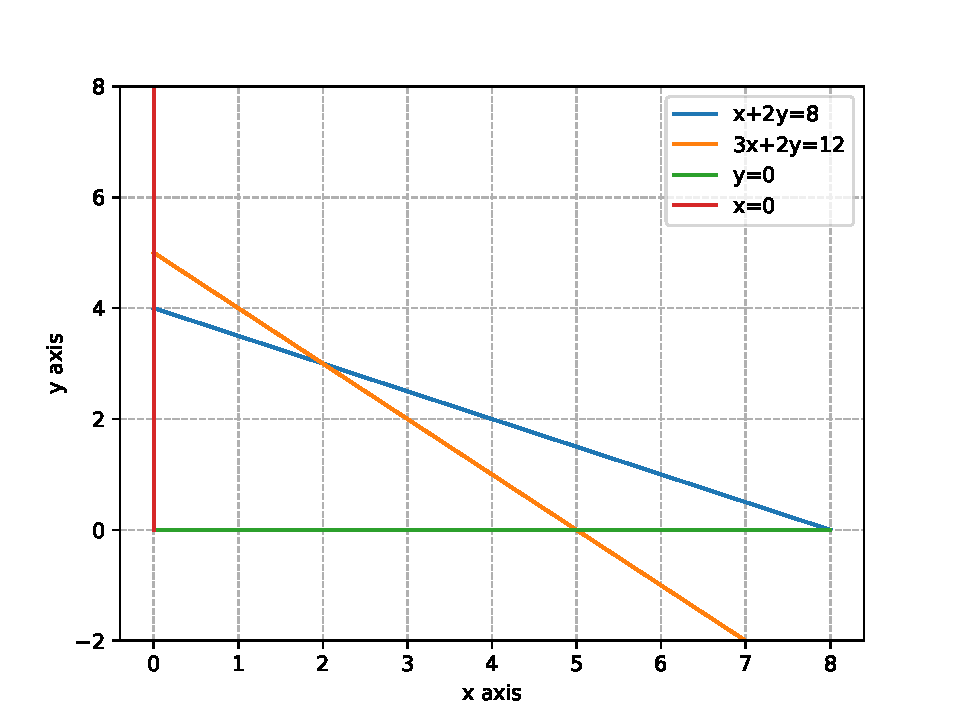
\includegraphics[width=\columnwidth]{12/12/1/2/figs/fig.pdf}
		\caption{}
		\label{fig:12/12/1/2}
  	\end{figure}
	\iffalse
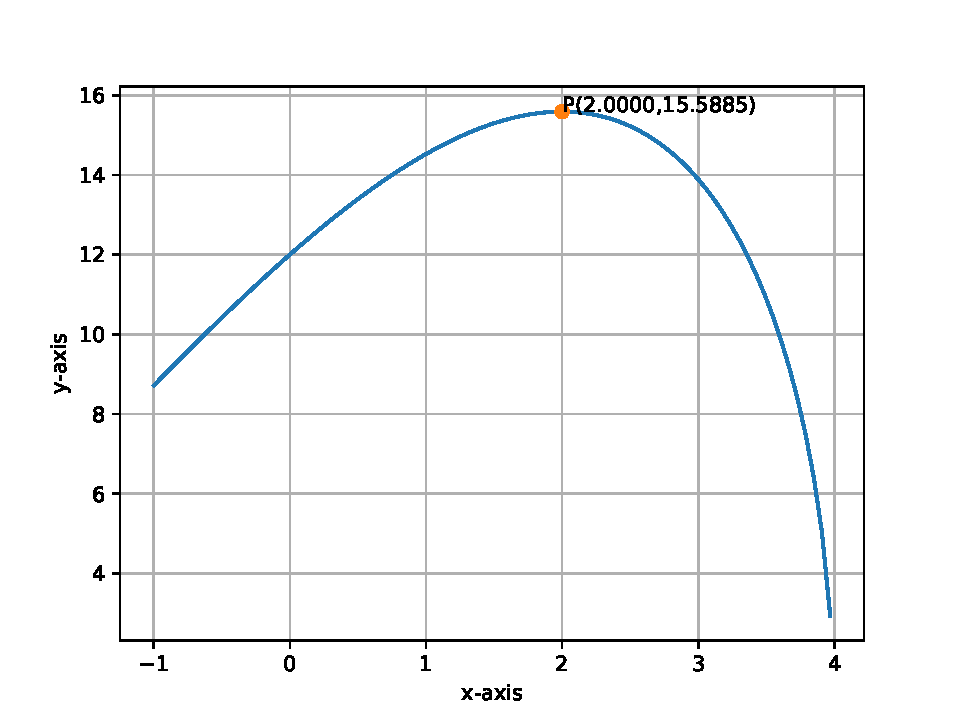
\includegraphics[scale=0.5]{fig.pdf} 
\end{flushleft}}
\section*{Solution}
\begin{flushleft}
	\fi
	The given
problem can be formulated as
\iffalse
\begin{align}
\min_{\vec{x}} Z=(-3x+4y)
\end{align}
\begin{align}
x+2y \preceq8
\end{align}
\begin{align}
3x+2y \preceq 12
\end{align}
\begin{align}
x\succeq0,y\succeq0
\end{align}
eq 2 and 3 to 4 can be expressed in vector form as
\fi
\begin{align}
	\min_{\vec{x}}Z=\myvec{-3 & 4}\vec{x}\\
\myvec{1 & 2\\
       3 & 2\\
       1 &0\\
       0 & 1}\vec{x}\succeq \myvec{8 \\12\\0\\0}
\end{align}
Solving above equations using cvxpy, we get
\begin{align}
	\min_{\vec{x}} Z&=-12
	\\
	\vec{x}&=\myvec{4\\0}
\end{align}

\item
\label{12/12/1/3}
\iffalse
<<<<<<< HEAD
hi
=======
\documentclass[a4paper,12pt,twocolumn]{article}
\usepackage{graphicx}
\usepackage[margin=0.5in]{geometry}
\usepackage[cmex10]{amsmath}
\usepackage{array}
\usepackage{gensymb}
\usepackage{booktabs}
\title{Optimization Assignment}

\author{Ravi Sumanth Muppana- FWC22003}
\date{September 2022}
\providecommand{\norm}[1]{\left\lVert#1\right\rVert}
\providecommand{\abs}[1]{\left\vert#1\right\vert}
\let\vec\mathbf
\newcommand{\myvec}[1]{\ensuremath{\begin{pmatrix}#1\end{pmatrix}}}
\newcommand{\mydet}[1]{\ensuremath{\begin{vmatrix}#1\end{vmatrix}}}
\providecommand{\brak}[1]{\ensuremath{\left((#1\right)}}
\begin{document}
\maketitle
\section{Problem:}
\fi
Maximize $Z$ = $5x+3y$ such that 
\begin{align}
	3x+5y&\le15,
	\\
	5x+2y&\le10,
	\\
	x\ge0,y&\ge0.
\end{align}
\solution
\iffalse
	\begin{figure}[!ht]
		\centering
		\includegraphics[width=\columnwidth]{12/12/1/3/figs/optim.png}
		\caption{}
		\label{fig:12/12/1/3}
  	\end{figure}
\maketitle
\section{Solution:}
\begin{figure}[h]
\includegraphics[width=\linewidth]{optim.png}
        \caption{feasible region}
\end{figure}
The feasible region is shown in Fig.
		\ref{fig:12/12/1/3}.
\subsection{Theory:}
We need to first graph the feasible region of the system of inequalities.  The region is bounded. We need to find the coordinates of corner points and figure the minimum value of $Z$. The given set of equations are:
\begin{align}
	&3x+5y\le15\\
	&5x+2y\le10\\
	&x\ge0\\
	&y\ge0\\
\end{align}
In vector form, they are written as:
\fi
The given problem can be expressed as
\begin{align}
	Z =\myvec{5 & 3}\vec{x}
	\\
s.t. \quad	\myvec{3 & 5\\5&2}\vec{x}\le\myvec{15\\10}\\
	\myvec{1&0\\0&1}\vec{x}\ge\myvec{0\\0}\\
\end{align}
Using cvxpy, the 
solution is 
\iffalse
\subsection{Mathematical Calculation:}
We need to find the intersection of given system of inequalities, to figure out the coordinates of feasible region.
The coordinates of the quadrilateral are $\myvec{0\\3}$, $\myvec{0\\2}$, $\myvec{0\\0}$, $\myvec{\frac{20}{19} \\ \frac{45}{19}}$.
Solving using cvxpy, we get,
\fi
\begin{align}
	\vec{x} = \myvec{\frac{20}{19}\\\frac{45}{19}},
	Z_{max} = \frac{235}{19}
\end{align}
\iffalse
Hence, the maximum of Z is verified using optimization.
 
\section{Construction:}
The construction of system of equations can be done by plotting them using matplotlib library.
\begin{table}[h]
        \centering
\setlength\extrarowheight{2pt}
        \begin{tabular}{|c|c|c|}
                \hline
		\textbf{variable} & \textbf{equation} & \textbf{comments}\\
		\hline
		y1 & (15-3x)/5 & eqn 1\\
		\hline
		y2 & (10-5x)/5 & eq 2\\
		\hline
	\end{tabular}
\end{table}

\end{document}
>>>>>>> f531642 (Created codes and figs folder)
\fi

\item
\label{12/12/1/4}
\iffalse
\documentclass[a4paper,12pt,twocolumn]{article}
\usepackage{graphicx}
\usepackage[margin=0.5in]{geometry}
\usepackage[cmex10]{amsmath}
\usepackage{array}
\usepackage{gensymb}
\usepackage{booktabs}
\title{Optimization Assignment}

\author{Manideep Parusha- FWC22004}
\date{September 2022}
\providecommand{\norm}[1]{\left\lVert#1\right\rVert}
\providecommand{\abs}[1]{\left\vert#1\right\vert}
\let\vec\mathbf
\newcommand{\myvec}[1]{\ensuremath{\begin{pmatrix}#1\end{pmatrix}}}
\newcommand{\mydet}[1]{\ensuremath{\begin{vmatrix}#1\end{vmatrix}}}
\providecommand{\brak}[1]{\ensuremath{\left((#1\right)}}
\begin{document}
\maketitle
\section{Problem:}
\fi
Minimize $Z$ = $3x+5y$ such that 
\begin{align}
x+3y&\ge3
\\
x+y&\ge2
\\
x\ge0, y&\ge0.
\end{align}
\solution
\iffalse
\maketitle
\section{Solution:}
%\subsection{Theory:}
We need to first graph the feasible region of the system of inequalities. The feasible region is shown in the above figure in color red. The region is bounded. We need to find the coordinates of corner points and figure the minimum value of $Z$. The given set of equations are:
\begin{align}
	x+3y\ge3\\
	x+y\ge2\\
	x\ge0\\
	y\ge0
\end{align}
\fi
The given problem can be expressed as
\begin{align}
	Z = \min_{\vec{x}}\myvec{3 & 5}\vec{x}
	\\
	\myvec{1 & 3\\1&1}\vec{x}\succeq\myvec{3\\2}\\
	\myvec{1&0\\0&1}\vec{x}\succeq\myvec{0\\0}
\end{align}
\iffalse
%\subsection{Mathematical Calculation:}
We need to find the intersection of given system of inequalities, to figure out the coordinates of feasible region.
The coordinates of the quadrilateral are $\myvec{0\\2}$, $\myvec{\frac{3}{2}\\\frac{1}{2}}$, $\myvec{3\\0}$.
\fi
Solving using cvxpy, we get,
\begin{align}
	\vec{x} = \myvec{\frac{3}{2}\\\frac{1}{2}},
	Z_{min} = 7
\end{align}
\iffalse
Hence, the minimum of Z is verified using optimization.
 
%\section{Construction:}
%The construction of system of equations can be done by plotting them using matplotlib library.
%\begin{table}[h]
 %       \centering
%\setlength\extrarowheight{2pt}
 %       \begin{tabular}{|c|c|c|}
  %              \hline
%		\textbf{variable} & \textbf{equation} & \textbf{comments}\\
%		\hline
%		y1 & (3-x)/3 & eqn 1\\
%		\hline
%		y2 & (2-x) & eq 2\\
%		\hline
%	\end{tabular}
%\end{table}

\end{document}
\fi

\item
\label{12/12/1/5}
%\iffalse
\documentclass[journal,10pt,twocolumn]{article}
\usepackage{graphicx}
\usepackage[margin=0.5in]{geometry}
\usepackage{amsmath}
\usepackage{array}
\usepackage{booktabs}
\usepackage{listings}
\providecommand{\norm}[1]{\left\lVert#1\right\rVert}
\providecommand{\abs}[1]{\left\vert#1\right\vert}
\usepackage{enumerate}
\let\vec\mathbf
\newcommand{\myvec}[1]{\ensuremath{\myvec{#1}}}
\newcommand{\mydet}[1]{\ensuremath{\begin{vmatrix}#1\end{vmatrix}}}
\providecommand{\brak}[1]{\ensuremath{\left(#1\right)}}
\lstset{
frame=single,
breaklines=true,
columns=fullflexible
}
\title{\textbf{Matrix Assignment}}
\author{Mannava Venkatasai}
\date{September 2022}
\begin{document}
\maketitle
\raggedright \textbf{Problem Statement}: \vspace{3mm} \\
Two godowns A and B have grain capacity of 100 quintals and 50 quintals
respectively. They supply to 3 ration shops, D, E and F whose requirements are
60, 50 and 40 quintals respectively. The cost of transportation per quintal from
the godowns to the shops are given in the following table
\begin{table}[!ht]
	\centering
\begin{tabular}{|c|c|c|}
\hline
% \begin{tabularx}{\linewidth} {lX}
 From/to & A& B  \\ 
 \hline
 D & 6 & 4 \\  
 \hline
 E & 3  & 2 \\
 \hline
  F & 2.5 & 3 \\
 \hline
\end{tabular} 
\end{table} 
\vspace{5mm}
How should the supplies be transported in order that the transportation cost is minimum? What is the minimum cost?
\fi
%\\
%\solution
Let's assume that 
\begin{enumerate}
\item A supplies $x$ quintals grain to ration shop D.
\item A supplies $y$ quintals grain to ration shop E.
\item A will supply remaining grains 100-$x$-$y$ quintals to F.
\item B will supply 60-$x$ quintals grain to ration shop D. 
\item B will supply 50-$y$ quintals grain to ration shop E.
\item B will supply $x$+$y$-60 quintals grain to ration shop F.
\end{enumerate}
Total transportation cost is given by :
\begin{align}
P=2.5x+1.5y+410
\end{align}
Now, Since godown A can supply maximum 60 quintals to ration shop D and 50 quintals to ration shop E and have maximum 100 quintals capacity to supply.\vspace{2mm} \\ Also, if godown A supplies all 40 quintals to ration shop F, then remaining 60 quintals will be supplied to ration shop D and E and $x$ and $y$ is amount of grains. It can never be negative.  This leads to the following conditions
\begin{align}
x+y \le 100 \\
x \le 60 \\
y \le 50 \\
-x-y \le -60 \\
x \ge 0 \\
y \ge 0
\end{align}
\iffalse
The above equations in vector form is :
\begin{align}
\vec{A_1} = 
\myvec{
1 \\
1 \\
} \\
\vec{A_2} = 
\myvec{
1 \\
1 \\
} \\
\vec{A_3} = 
\myvec{
1 \\
0 \\
} \\
\vec{A_4} = 
\myvec{
0 \\
1 \\
} \\
\vec{x} = 
\myvec{
x \\
y \\
}
\end{align}
\begin{align}
\vec{A_1}\vec{x} \le 100
\end{align}
\begin{align}
\vec{A_2}\vec{x} \ge 60
\end{align}
\begin{align}
\vec{A_3}\vec{x} \le 60
\end{align}
\begin{align}
\vec{A_4}\vec{x} \le 50
\end{align}
which can be expressed in vector form as
\fi
The optimization problem can then be expressed as
\begin{align}
	P=\max_{\vec{x}}\myvec{2.5 & 1.5}\vec{x}+410
	\\
	s.t. \quad
 \myvec{1 &1 \\ -1 & -1 \\ -1 & 0 \\ 0 & -1 \\} \vec{x}\preceq \myvec{100 \\ -60 \\ -60 \\ -50}
\end{align}
yielding
\begin{align}
	P = 510, 
\vec{x} = 
\myvec{
10 \\
50 \\
}
\end{align}
Hence,
\begin{enumerate}
\item The minimum transportation cost is : 510 /-
\item A supplies 10 quintals grain to ration shop D.
\item A supplies 50 quintals grain to ration shop E.
\item A supplies 40 quintals grain to ration shop F.
\item A supplies 50 quintals grain to ration shop D.
\item A supplies 0 quintals grain to ration shop E.
\item A supplies 0 quintals grain to ration shop F.
\end{enumerate}

\item
\label{12/12/1/6}
\iffalse
\documentclass[a4paper,12pt,twocolumn]{article}
\usepackage{graphicx}
\usepackage[margin=0.5in]{geometry}
\usepackage[cmex10]{amsmath}
\usepackage{array}
\usepackage{gensymb}
\usepackage{booktabs}
\usepackage{tabularx}
\title{Conic Assignment}

\author{Ginna Shreyani- FWC22006}
\date{October 2022}
\providecommand{\norm}[1]{\left\lVert#1\right\rVert}
\providecommand{\abs}[1]{\left\vert#1\right\vert}
\let\vec\mathbf
\newcommand{\myvec}[1]{\ensuremath{\begin{pmatrix}#1\end{pmatrix}}}
\newcommand{\mydet}[1]{\ensuremath{\begin{vmatrix}#1\end{vmatrix}}}
\providecommand{\brak}[1]{\ensuremath{\left((#1\right)}}
\begin{document}
\maketitle											
\section{Problem:}
\fi
Minimize Z=x+2y subject to
\begin{align}
	2x+3y&\ge3
	\\
	x+2y&\ge6
	\\
	x,y&\ge0.
\end{align}
\solution
	\begin{figure}[!ht]
		\centering
		\includegraphics[width=\columnwidth]{12/12/1/6/figs/optimize.png}
		\caption{}
		\label{fig:12/12/1/6}
  	\end{figure}
	\iffalse
\maketitle
\section{Solution:}
The given equations are
\begin{align*}
&2x+y\ge3\\
&x+2y\ge6\\
&x,y\ge0\\
\end{align*}
\begin{figure}[h]
     \includegraphics[width=\linewidth]{figures/optimize.png}
\end{figure}
By solving the above equations we get that feasible region of  these two equations is unbounded.Here, the red unbounded region is the feasible region of the above given equations. Here the feasible region is unbounded, so the minimum value of $\vec{Z}$ is found by finding the corner points.\\
\fi
The optimization problem can be defined as
\begin{align}
	P = \min_{\vec{x}}\myvec{1 &2}\vec{x}
	\\
	\myvec{2 &1 \\ 1 & 2} \vec{x}\succeq \myvec{3 \\ 6}
	\\
x,y \ge \vec{0}
\end{align}
From Fig. 
		\ref{fig:12/12/1/6},
 %Graphical solution:} 
				the feasible region vertices are
\begin{align}
\myvec{0 \\ 3 },
\myvec{6 \\ 0}
\end{align}
yielding
\begin{align}
	\myvec{1 &2}\myvec{0 \\ 3} &= 6 \\
	\myvec{1 &2}\myvec{6 \\ 0} &= 6 \\
	%\myvec{30 &20}\myvec{4 \\ 12} &= 360
\end{align}
Thus, the minimum value of Z is 6.
%along the line $\myvec{1 & 2}\vec{x}=\myvec{6 \\ 0}$.

\item
\label{12/12/1/7}
\iffalse
\documentclass{article}
% Language setting
% Replace `english' with e.g. `spanish' to change the document language
\usepackage[english]{babel}
% Set page size and margins
% Replace `letterpaper' with `a4paper' for UK/EU standard size
\usepackage[letterpaper,top=2cm,bottom=2cm,left=3cm,right=3cm,marginparwidth=1.75cm]{geometry}
% Useful packages
\usepackage{multicol}
\usepackage{amsmath}
\usepackage{amssymb}
\usepackage{graphicx}
\usepackage[framemethod=tikz]{mdframed}
\usepackage{array}
\usepackage{blindtext}
%\usepackage[paperwidth=10cm]{geometry}
\usepackage{tkz-euclide}
%\usepackage{tikz}
\usetikzlibrary{
  circuits.logic,
  circuits.logic.US,
  positioning
}

\usepackage[colorlinks=true, allcolors=blue]{hyperref}
\newcommand{\myvec}[1]{\ensuremath{\begin{pmatrix}#1\end{pmatrix}}}
\providecommand{\norm}[1]{\left\lVert#1\right\rVert}
\let\vec\mathbf
\title{Optimization Assignment-1}
\author{Ballepu dheeraj kumar}
\begin{document}
\maketitle
\newtheorem{theorem}{Theorem}[section]
\begin{multicols}{2}

\paragraph{\begin{flushleft}\textbf{Problem: }
\fi
Minimise and Maximise
\begin{align}
Z = 5x+10y
\end{align}
subject to
\begin{align}
	x+2y &\le 120
	\\
	x+y &\ge 60
	\\
	x-2y &\ge 0
	\\
	x \ge 0 , y &\ge 0
\end{align}
\solution
	\begin{figure}[!ht]
		\centering
		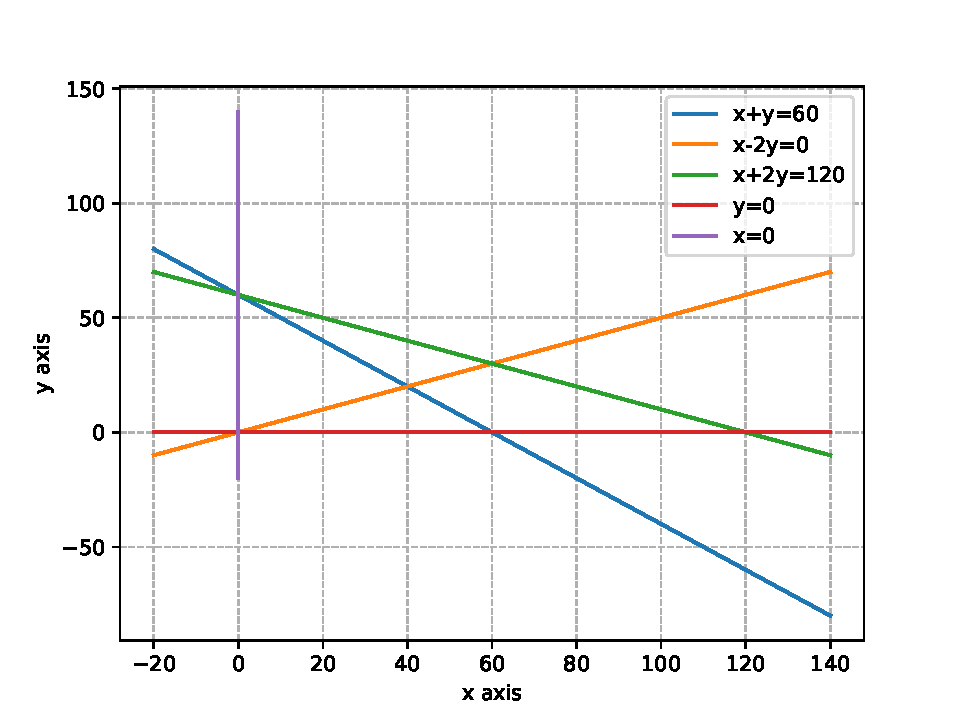
\includegraphics[width=\columnwidth]{12/12/1/7/figs/opt1.pdf}
		\caption{}
		\label{fig:12/12/1/7}
  	\end{figure}
	\iffalse
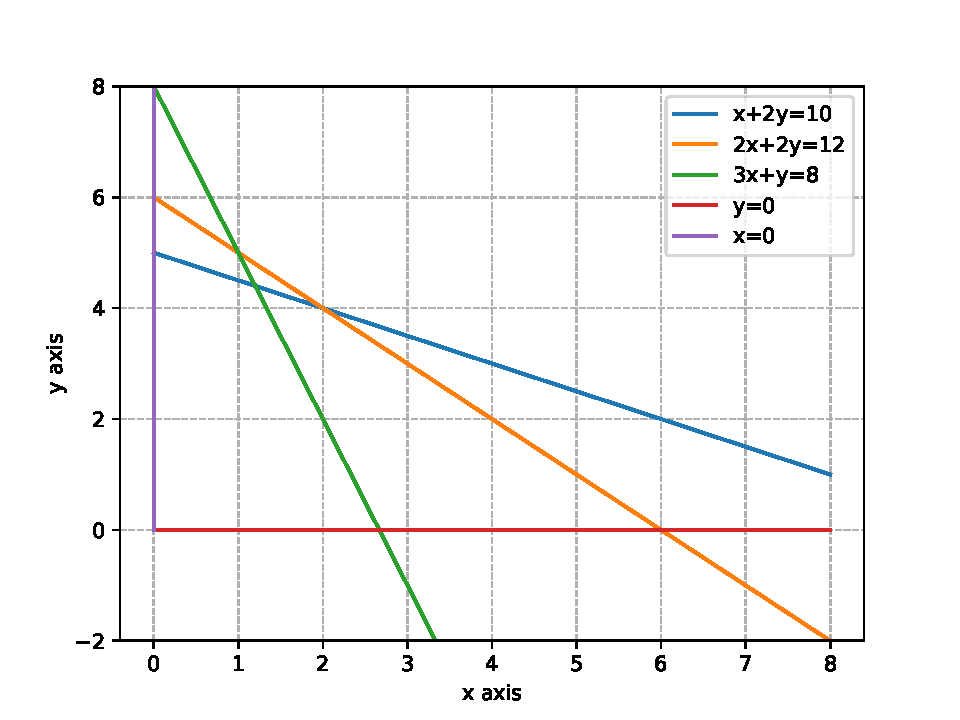
\includegraphics[scale=0.5]{/sdcard/Download/Opti/figure2/opt1.pdf} 
\end{flushleft}}
\section*{Solution}
\begin{flushleft}
\begin{align}
\min_{\vec{x}} Z=(5x+10y)\\
\max_{\vec{x}} Z=(5x+10y) \\
\end{align}
\begin{align*}
x+2y \preceq 120
\end{align*}
\begin{align*}
x+y \succeq 60
\end{align*}
\begin{align*}
x-2y \succeq 60
\end{align*}
\begin{align*}
x \succeq 0 , y \succeq 0
\end{align*}
all the above expressions can be expressed in vector form as
\fi
	The given 
problem can be formulated as
\begin{align}
	\min_{\vec{x}}\vec{Z}=\myvec{5 & 10}\vec{x}\\
	\max_{\vec{x}}\vec{Z}=\myvec{5 &10}\vec{x}\\
	s.t. \quad
	\myvec{
	-1 & -2 \\
		1 &1\\
	1 & -2\\
	1 &0\\
	0 &1
	}\vec{x}\succeq \myvec{-120 \\ 60 \\0\\0\\0}\\   
\end{align}
%\begin{align}
%\max_{\vec{x}}\vec{Z}=\myvec{5 \hspace{0.2cm}10}\vec{x}\\
%\myvec{1 \hspace{0.2cm}2\vec{x}\preceq \myvec{120}
%\end{align}
Solving above equations using cvxpy,
\begin{align}
\min_{\vec{x}} Z=300,
\vec{x}=\myvec{60\\0}
\\
\max_{\vec{x}} Z=600,
\vec{x}=\myvec{60\\30}
\end{align}
\iffalse
\end{multicols}{2}
\end{document}
\fi

\item
\label{12/12/1/8}
%\iffalse
\documentclass[journal,10pt,twocolumn]{article}
\usepackage{graphicx}
\usepackage[margin=0.5in]{geometry}
\usepackage{amsmath}
\usepackage{array}
\usepackage{booktabs}
\usepackage{listings}
\providecommand{\norm}[1]{\left\lVert#1\right\rVert}
\providecommand{\abs}[1]{\left\vert#1\right\vert}
\usepackage{enumerate}
\let\vec\mathbf
\newcommand{\myvec}[1]{\ensuremath{\myvec{#1}}}
\newcommand{\mydet}[1]{\ensuremath{\begin{vmatrix}#1\end{vmatrix}}}
\providecommand{\brak}[1]{\ensuremath{\left(#1\right)}}
\lstset{
frame=single,
breaklines=true,
columns=fullflexible
}
\title{\textbf{Matrix Assignment}}
\author{Mannava Venkatasai}
\date{September 2022}
\begin{document}
\maketitle
\raggedright \textbf{Problem Statement}: \vspace{3mm} \\
Two godowns A and B have grain capacity of 100 quintals and 50 quintals
respectively. They supply to 3 ration shops, D, E and F whose requirements are
60, 50 and 40 quintals respectively. The cost of transportation per quintal from
the godowns to the shops are given in the following table
\begin{table}[!ht]
	\centering
\begin{tabular}{|c|c|c|}
\hline
% \begin{tabularx}{\linewidth} {lX}
 From/to & A& B  \\ 
 \hline
 D & 6 & 4 \\  
 \hline
 E & 3  & 2 \\
 \hline
  F & 2.5 & 3 \\
 \hline
\end{tabular} 
\end{table} 
\vspace{5mm}
How should the supplies be transported in order that the transportation cost is minimum? What is the minimum cost?
\fi
%\\
%\solution
Let's assume that 
\begin{enumerate}
\item A supplies $x$ quintals grain to ration shop D.
\item A supplies $y$ quintals grain to ration shop E.
\item A will supply remaining grains 100-$x$-$y$ quintals to F.
\item B will supply 60-$x$ quintals grain to ration shop D. 
\item B will supply 50-$y$ quintals grain to ration shop E.
\item B will supply $x$+$y$-60 quintals grain to ration shop F.
\end{enumerate}
Total transportation cost is given by :
\begin{align}
P=2.5x+1.5y+410
\end{align}
Now, Since godown A can supply maximum 60 quintals to ration shop D and 50 quintals to ration shop E and have maximum 100 quintals capacity to supply.\vspace{2mm} \\ Also, if godown A supplies all 40 quintals to ration shop F, then remaining 60 quintals will be supplied to ration shop D and E and $x$ and $y$ is amount of grains. It can never be negative.  This leads to the following conditions
\begin{align}
x+y \le 100 \\
x \le 60 \\
y \le 50 \\
-x-y \le -60 \\
x \ge 0 \\
y \ge 0
\end{align}
\iffalse
The above equations in vector form is :
\begin{align}
\vec{A_1} = 
\myvec{
1 \\
1 \\
} \\
\vec{A_2} = 
\myvec{
1 \\
1 \\
} \\
\vec{A_3} = 
\myvec{
1 \\
0 \\
} \\
\vec{A_4} = 
\myvec{
0 \\
1 \\
} \\
\vec{x} = 
\myvec{
x \\
y \\
}
\end{align}
\begin{align}
\vec{A_1}\vec{x} \le 100
\end{align}
\begin{align}
\vec{A_2}\vec{x} \ge 60
\end{align}
\begin{align}
\vec{A_3}\vec{x} \le 60
\end{align}
\begin{align}
\vec{A_4}\vec{x} \le 50
\end{align}
which can be expressed in vector form as
\fi
The optimization problem can then be expressed as
\begin{align}
	P=\max_{\vec{x}}\myvec{2.5 & 1.5}\vec{x}+410
	\\
	s.t. \quad
 \myvec{1 &1 \\ -1 & -1 \\ -1 & 0 \\ 0 & -1 \\} \vec{x}\preceq \myvec{100 \\ -60 \\ -60 \\ -50}
\end{align}
yielding
\begin{align}
	P = 510, 
\vec{x} = 
\myvec{
10 \\
50 \\
}
\end{align}
Hence,
\begin{enumerate}
\item The minimum transportation cost is : 510 /-
\item A supplies 10 quintals grain to ration shop D.
\item A supplies 50 quintals grain to ration shop E.
\item A supplies 40 quintals grain to ration shop F.
\item A supplies 50 quintals grain to ration shop D.
\item A supplies 0 quintals grain to ration shop E.
\item A supplies 0 quintals grain to ration shop F.
\end{enumerate}

\item
\label{12/12/1/9}
\iffalse
\def\mytitle{Convex-Optimization}
\def\myauthor{K.Pavan Kumar}
\def\contact{r170850@rguktrkv.ac.in}
\def\mymodule{Future Wireless Communication (FWC)}
\documentclass[10pt, a4paper]{article}
\usepackage[a4paper,outer=1.5cm,inner=1.5cm,top=1.75cm,bottom=1.5cm]{geometry}
\twocolumn
\usepackage{graphicx}
\graphicspath{{./images/}}
\usepackage[colorlinks,linkcolor={black},citecolor={blue!80!black},urlcolor={blue!80!black}]{hyperref}
\usepackage[parfill]{parskip}
\usepackage{lmodern}
\usepackage{tikz}
	\usepackage{physics}
\usepackage{tabularx}
\usepackage{enumitem}
\usetikzlibrary{calc}
\usepackage{amsmath}
\usepackage{amssymb}
\renewcommand*\familydefault{\sfdefault}
\usepackage{watermark}
\usepackage{lipsum}
\usepackage{xcolor}
\usepackage{listings}
\usepackage{float}
\usepackage{titlesec}
\providecommand{\mtx}[1]{\mathbf{#1}}
\titlespacing{\subsection}{1pt}{\parskip}{3pt}
\titlespacing{\subsubsection}{0pt}{\parskip}{-\parskip}
\titlespacing{\paragraph}{0pt}{\parskip}{\parskip}


\newcommand{\myvec}[1]{\ensuremath{\begin{pmatrix}#1\end{pmatrix}}}
\let\vec\mathbf
\lstset{
frame=single, 
breaklines=true,
columns=fullflexible
}
\thiswatermark{\centering \put(0,-110.0){
\includegraphics[scale=0.3]{logo.png}} }
\title{\mytitle}
\author{\myauthor\hspace{1em}\\\contact\\FWC22011\hspace{6.5em}IITH\hspace{0.5em}\mymodule\hspace{6em}Optimization:Basic}
\date{}
\begin{document}
	\maketitle
	\tableofcontents
   \section{Problem}
   \fi
Maximise 
\begin{align}
Z = – x + 2y
\end{align}
 subject to the constraints
\begin{align}
	x + y &\geq 5
	\\
	x + 2y &\geq 6
	\\
	x \geq 3, y &\geq 0.
\end{align}
	\begin{figure}[!ht]
		\centering
		\includegraphics[width=\columnwidth]{12/12/1/9/figs/image.png}
		\caption{}
		\label{fig:12/12/1/9}
  	\end{figure}
\solution
The given problem can be expressed as
\begin{align}
z = \max_\vec{x}\myvec{-1 &2}\vec{x}
\\
s.t. \quad
    \myvec{1&1\\1&2\\1&0\\0&1}\vec{x}=\myvec{5\\6\\3\\0}
\end{align}
By providing the objective function and constraints to cvxpy, the optimal value gives infinity as result and the problem is unbounded.
This is verified from Fig. 
		\ref{fig:12/12/1/9}.
		\iffalse

\textbf{Reason:}
Unbounded means  if there exists some direction within the feasible region along which the objective function value can increase (maximization case) or decrease (minimization case) without bound. In such a formulation, the optimal value is negative infinity for a minimization problem, and conversely, positive infinity for a maximization problem.

An unbounded solution is something that typically does not arise in practical applications. When it does occur, it’s usually because the formulation is ill-posed, i.e., incorrect in some way, and/or missing some necessary constraints for properly modeling the dynamics of the system under consideration.

\vspace{20cm}
\textbf{termux commands :}
\begin{lstlisting}
bash basic.sh............using shell command
\end{lstlisting}

\textbf{cvxpy code:}
\begin{center}
\fbox{\parbox{8.5cm}{\url{https://github.com/FWC_module1/blob/main/optimization/basic.py}}}
\end{center}

\textbf{Graphical method:}
\begin{center}
   {\includegraphics[scale=0.5]{image.png}}  
\end{center}
From Graph,
\begin{center}
\begin{tabular}{|c|c|}
	\hline
	corner points&z\\
	\hline
	\textbf{(3,2)}&\textbf{1}\\
	\hline
    (4,1)&-2\\
    \hline
    (6,0)&-6\\
	\hline
\end{tabular}
\end{center}

Clearly the corner point (3,2) has maximum value for the given objective function.

But, as the feasible region is unbounded ,'\textbf{1}' may or may not be the maximum value. So ,we need to graph the inequality -x+2y $>$ 1.\\
$\because$ Feasible region of -x+2y $>$ 1 has some  points in common with the given constraints .so ,there is no maximum value for  z subject to given constraints.

\end{document}
\fi

\item
\label{12/12/1/10}
\iffalse
\def\mytitle{OPTIMIZATION}
\def\myauthor{VUNNAVA SRAVANI}
\def\contact{sravani21vunnava@gmail.com}
\def\mymodule{Future Wireless Communication (FWC)}
\documentclass[10pt, a4paper]{article}
\usepackage[a4paper,outer=1.5cm,inner=1.5cm,top=1.75cm,bottom=1.5cm]{geometry}
\twocolumn
\usepackage{setspace}
\usepackage{graphicx}
\graphicspath{{./images/}}
\usepackage[colorlinks,linkcolor={black},citecolor={blue!80!black},urlcolor={blue!80!black}]{hyperref}
\usepackage[parfill]{parskip}
\usepackage{lmodern}
\usepackage{tikz}
	\usepackage{physics}
%\documentclass[tikz, border=2mm]{standalone}
\usepackage{karnaugh-map}
\usepackage{tabularx}
\usetikzlibrary{calc}
\usepackage{amsmath}
\usepackage{amssymb}
\renewcommand*\familydefault{\sfdefault}
\usepackage{watermark}
\usepackage{lipsum}
\usepackage{xcolor}
\usepackage{listings}
\usepackage{float}
\usepackage{titlesec}
\providecommand{\mtx}[1]{\mathbf{#1}}
\titlespacing{\subsection}{1pt}{\parskip}{3pt}
\titlespacing{\subsubsection}{0pt}{\parskip}{-\parskip}
\titlespacing{\paragraph}{0pt}{\parskip}{\parskip}
\newcommand{\figuremacro}[5]{//
    \begin{figure}[#1]
        \centering
        \includegraphics[width=#5\columnwidth]{#2}
        \caption[#3]{\textbf{#3}#4}
        \label{fig:#2}
    \end{figure}
}
\newcommand{\myvec}[1]{\ensuremath{\begin{pmatrix}#1\end{pmatrix}}}
\let\vec\mathbf
\lstset{
frame=single, 
breaklines=true,
columns=fullflexible
}

\title{\mytitle}
\author{\myauthor\hspace{1em}\\\contact\\FWC22012\hspace{6.5em}IITH\hspace{0.5em}\mymodule\hspace{6em}ASSIGN-8}
\date{}
\begin{document}
	\maketitle
	\tableofcontents

\section{Construction}
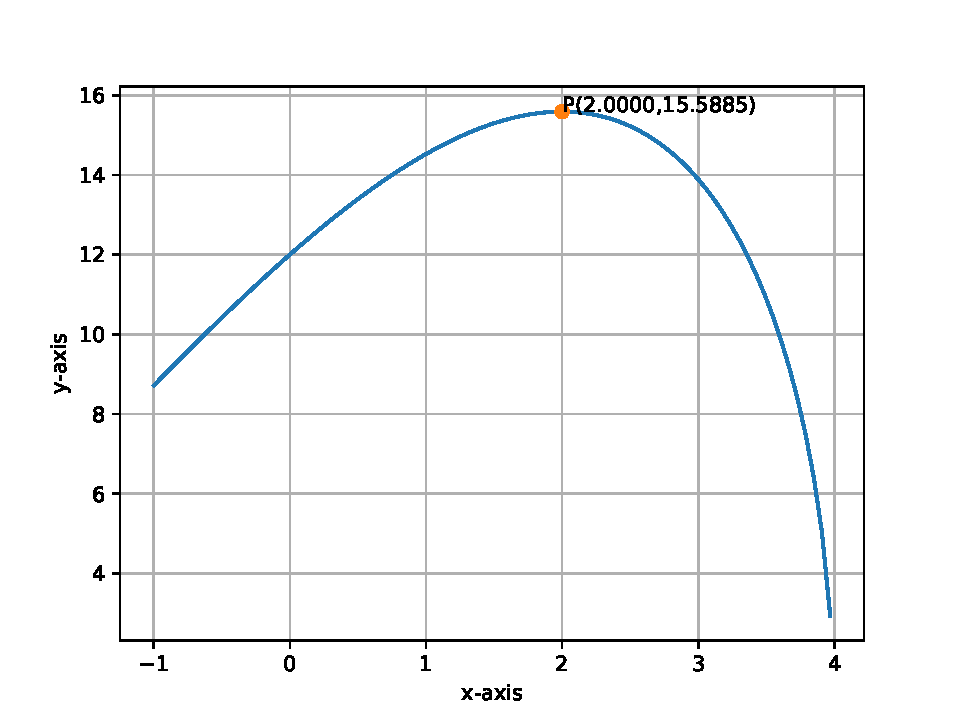
\includegraphics[scale=0.5]{fig.pdf}

\section{Problem}
\fi
Maximize 
\begin{align}
Z = x+y 
\end{align}
subject to
\begin{align}
 x - y &\le -1
	\\
	-x+y&\le0 
	\\
	x,y &\ge 0
\end{align}
\solution 
	\begin{figure}[!ht]
		\centering
		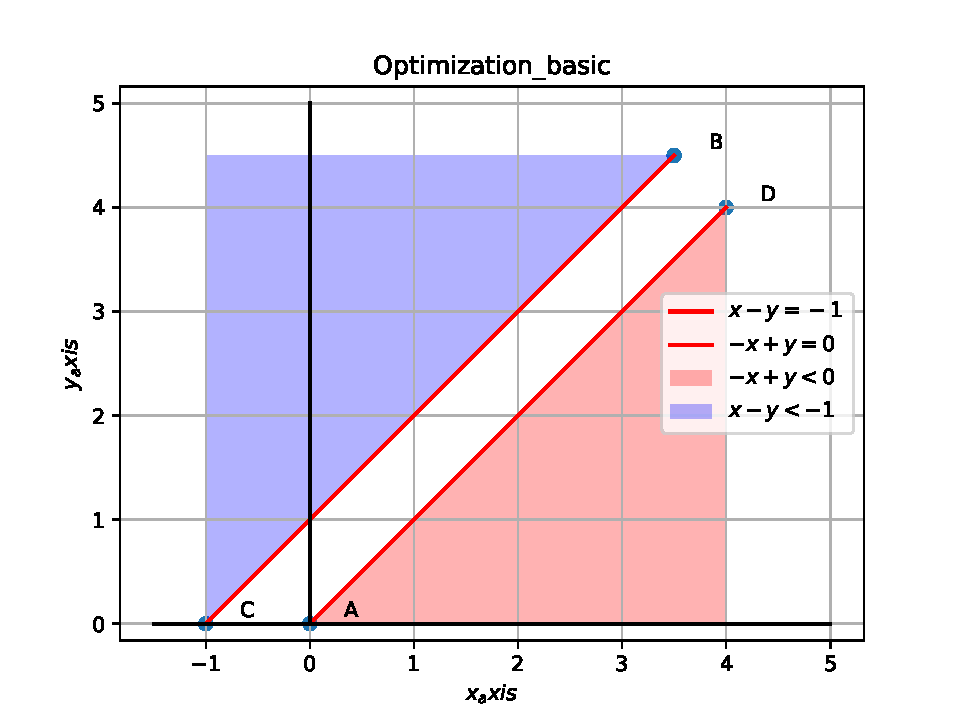
\includegraphics[width=\columnwidth]{12/12/1/10/figs/fig.pdf}
		\caption{}
		\label{fig:12/12/1/10}
  	\end{figure}
	From Fig. 
		\ref{fig:12/12/1/10},
		the given problem has no optimal solution.  This is verified from cvxpy by considering the following optimization problem.
	\iffalse
\section{Solution}
Consider,
\begin{tabular}{|c|c|}
	\hline
	\textbf{Parameter}&\textbf{Value}\\
	\hline
	$\vec{c}$ & $\myvec{1\\1}$ \\
	\hline
	$\vec{x}$ & $\myvec{x\\y}$ \\
	\hline
	$\vec{p}$ & $\myvec{1&-1 \\ -1&0 \\ 0&-1 \\ -1&0}$ \\
	\hline
\end{tabular}\\

Objective function:
Constraints:
\begin{align}
x - y\le -1
\end{align}
\begin{align}
-x + y \le 0
\end{align}
\begin{align}
-x \le 0
\end{align}
\begin{align}
-y \le 0
\end{align}
writing all the constraints in matrix form:
\begin{align}
\vec{p^T}\vec{x} \preceq \vec{q}
\end{align}
\fi
\begin{align}
	z = \max_{x}\myvec{1 & 1}\vec{x}
	\\
	s.t. \quad
\myvec{1&-1 \\ -1&0 \\ 0&-1 \\ -1&0}x \preceq \myvec{-1 \\ 0 \\ 0 \\ 0 }
\end{align}
\iffalse
By providing the objective function and constraints to cvxpy, we get the optimal solution for z
\\
\textbf{cvxpy code}

from cvxpy code,\\
There is no feasible region between,\\
Hence there is no maximum value for z.

\end{document}
\fi

\iffalse
\item
\label{12/12/1/1}
\iffalse
\documentclass[journal,10pt,twocolumn]{article}
\usepackage{graphicx}
\usepackage[margin=0.5in]{geometry}
\usepackage{amsmath}
\usepackage{array}
\usepackage{booktabs}
\usepackage{listings}
\providecommand{\norm}[1]{\left\lVert#1\right\rVert}
\providecommand{\abs}[1]{\left\vert#1\right\vert}
\usepackage{enumerate}
\let\vec\mathbf
\newcommand{\myvec}[1]{\ensuremath{\myvec{#1}}}
\newcommand{\mydet}[1]{\ensuremath{\begin{vmatrix}#1\end{vmatrix}}}
\providecommand{\brak}[1]{\ensuremath{\left(#1\right)}}
\lstset{
frame=single,
breaklines=true,
columns=fullflexible
}
\title{\textbf{Matrix Assignment}}
\author{Mannava Venkatasai}
\date{September 2022}
\begin{document}
\maketitle
\raggedright \textbf{Problem Statement}: \vspace{3mm} \\
Two godowns A and B have grain capacity of 100 quintals and 50 quintals
respectively. They supply to 3 ration shops, D, E and F whose requirements are
60, 50 and 40 quintals respectively. The cost of transportation per quintal from
the godowns to the shops are given in the following table
\begin{table}[!ht]
	\centering
\begin{tabular}{|c|c|c|}
\hline
% \begin{tabularx}{\linewidth} {lX}
 From/to & A& B  \\ 
 \hline
 D & 6 & 4 \\  
 \hline
 E & 3  & 2 \\
 \hline
  F & 2.5 & 3 \\
 \hline
\end{tabular} 
\end{table} 
\vspace{5mm}
How should the supplies be transported in order that the transportation cost is minimum? What is the minimum cost?
\fi
%\\
%\solution
Let's assume that 
\begin{enumerate}
\item A supplies $x$ quintals grain to ration shop D.
\item A supplies $y$ quintals grain to ration shop E.
\item A will supply remaining grains 100-$x$-$y$ quintals to F.
\item B will supply 60-$x$ quintals grain to ration shop D. 
\item B will supply 50-$y$ quintals grain to ration shop E.
\item B will supply $x$+$y$-60 quintals grain to ration shop F.
\end{enumerate}
Total transportation cost is given by :
\begin{align}
P=2.5x+1.5y+410
\end{align}
Now, Since godown A can supply maximum 60 quintals to ration shop D and 50 quintals to ration shop E and have maximum 100 quintals capacity to supply.\vspace{2mm} \\ Also, if godown A supplies all 40 quintals to ration shop F, then remaining 60 quintals will be supplied to ration shop D and E and $x$ and $y$ is amount of grains. It can never be negative.  This leads to the following conditions
\begin{align}
x+y \le 100 \\
x \le 60 \\
y \le 50 \\
-x-y \le -60 \\
x \ge 0 \\
y \ge 0
\end{align}
\iffalse
The above equations in vector form is :
\begin{align}
\vec{A_1} = 
\myvec{
1 \\
1 \\
} \\
\vec{A_2} = 
\myvec{
1 \\
1 \\
} \\
\vec{A_3} = 
\myvec{
1 \\
0 \\
} \\
\vec{A_4} = 
\myvec{
0 \\
1 \\
} \\
\vec{x} = 
\myvec{
x \\
y \\
}
\end{align}
\begin{align}
\vec{A_1}\vec{x} \le 100
\end{align}
\begin{align}
\vec{A_2}\vec{x} \ge 60
\end{align}
\begin{align}
\vec{A_3}\vec{x} \le 60
\end{align}
\begin{align}
\vec{A_4}\vec{x} \le 50
\end{align}
which can be expressed in vector form as
\fi
The optimization problem can then be expressed as
\begin{align}
	P=\max_{\vec{x}}\myvec{2.5 & 1.5}\vec{x}+410
	\\
	s.t. \quad
 \myvec{1 &1 \\ -1 & -1 \\ -1 & 0 \\ 0 & -1 \\} \vec{x}\preceq \myvec{100 \\ -60 \\ -60 \\ -50}
\end{align}
yielding
\begin{align}
	P = 510, 
\vec{x} = 
\myvec{
10 \\
50 \\
}
\end{align}
Hence,
\begin{enumerate}
\item The minimum transportation cost is : 510 /-
\item A supplies 10 quintals grain to ration shop D.
\item A supplies 50 quintals grain to ration shop E.
\item A supplies 40 quintals grain to ration shop F.
\item A supplies 50 quintals grain to ration shop D.
\item A supplies 0 quintals grain to ration shop E.
\item A supplies 0 quintals grain to ration shop F.
\end{enumerate}

\fi
\end{enumerate}
